\documentclass[xelatex,aspectratio=169]{beamer}

\hfuzz=10pt
\vfuzz=10pt

% Theme
\usetheme{htw}
\setbeamertemplate{navigation symbols}{}
\setbeamertemplate{theorems}[numbered]
\setbeamercovered{transparent}

%\logo{
\includegraphics[height=0.5cm]{HTWD_color.png}}

% Packages
\usepackage{polyglossia}
\setmainlanguage{german}
\setotherlanguage{english}

\usepackage[bigfiles]{pdfbase}
\ExplSyntaxOn
\NewDocumentCommand\embedvideo{smm}{
\group_begin:
\leavevmode
\tl_if_exist:cTF{file_\file_mdfive_hash:n{#3}}{
  \tl_set_eq:Nc\video{file_\file_mdfive_hash:n{#3}}
}{
  \IfFileExists{#3}{}{\GenericError{}{File~`#3'~not~found}{}{}}
  \pbs_pdfobj:nnn{}{fstream}{{}{#3}}
  \pbs_pdfobj:nnn{}{dict}{
    /Type/Filespec/F~(#3)/UF~(#3)
    /EF~<</F~\pbs_pdflastobj:>>
  }
  \tl_set:Nx\video{\pbs_pdflastobj:}
  \tl_gset_eq:cN{file_\file_mdfive_hash:n{#3}}\video
}
%
\pbs_pdfobj:nnn{}{dict}{
  /Type/RichMediaInstance/Subtype/Video
  /Asset~\video
  /Params~<</FlashVars (
  source=#3&
  skin=SkinOverAllNoFullNoCaption.swf&
  skinAutoHide=true&
  skinBackgroundColor=0x5F5F5F&
  skinBackgroundAlpha=0.75
  )>>
}
%
\pbs_pdfobj:nnn{}{dict}{
/Type/RichMediaConfiguration/Subtype/Video
/Instances~[\pbs_pdflastobj:]
}
%
\pbs_pdfobj:nnn{}{dict}{
/Type/RichMediaContent
/Assets~<<
/Names~[(#3)~\video]
>>
/Configurations~[\pbs_pdflastobj:]
}
\tl_set:Nx\rmcontent{\pbs_pdflastobj:}
%
\pbs_pdfobj:nnn{}{dict}{
  /Activation~<<
  /Condition/\IfBooleanTF{#1}{PV}{XA}
  /Presentation~<</Style/Embedded>>
  >>
  /Deactivation~<</Condition/PI>>
}
%
\hbox_set:Nn\l_tmpa_box{#2}
\tl_set:Nx\l_box_wd_tl{\dim_use:N\box_wd:N\l_tmpa_box}
\tl_set:Nx\l_box_ht_tl{\dim_use:N\box_ht:N\l_tmpa_box}
\tl_set:Nx\l_box_dp_tl{\dim_use:N\box_dp:N\l_tmpa_box}
\pbs_pdfxform:nnnnn{1}{1}{}{}{\l_tmpa_box}
%
\pbs_pdfannot:nnnn{\l_box_wd_tl}{\l_box_ht_tl}{\l_box_dp_tl}{
  /Subtype/RichMedia
  /BS~<</W~0/S/S>>
  /Contents~(embedded~video~file:#3)
  /NM~(rma:#3)
  /AP~<</N~\pbs_pdflastxform:>>
  /RichMediaSettings~\pbs_pdflastobj:
  /RichMediaContent~\rmcontent
}
\phantom{#2}
\group_end:
}
\ExplSyntaxOff


\usepackage{graphicx}
\usepackage[export]{adjustbox}
\usepackage{animate}
%\usepackage[dvipdfmx]{movie15_dvipdfmx}
\usepackage{media9}
\usepackage{tabularx}
\usepackage{colortbl}
\usepackage{booktabs}
\usepackage{makecell}
\usepackage{ltablex}
\usepackage{array}
\usepackage{multirow}
\usepackage{amsmath}
\usepackage{amsthm}
%\renewcommand{\arraystretch}{1.5}
\newcolumntype{L}[1]{>{\raggedright\let\newline\\\arraybackslash\hspace{0pt}}p{#1}}
\newcolumntype{C}[1]{>{\centering\let\newline\\\arraybackslash\hspace{0pt}}p{#1}}
\newcolumntype{R}[1]{>{\raggedleft\let\newline\\\arraybackslash\hspace{0pt}}p{#1}}
%\renewcommand\thesatz{\arabic{section}.\arabic{theorem}}
\makeatletter
\@addtoreset{theorem}{lecture}
\makeatother

\newtheorem{satz}{Satz}[section]
\newtheorem{lem}{Lemma}[section]
\newtheorem{beh}{Behauptung}[section]
\newtheorem{define}{Definition}[section]
\numberwithin{equation}{section}
\usepackage{ragged2e}
\usepackage{etoolbox}

\usepackage{color}
\usepackage{colortbl}
\definecolor{hellgrau}{rgb}{0.85,0.85,0.85}
\definecolor{hellrot}{rgb}{1,0.7,0.7}

\usepackage{tikz}
\usetikzlibrary{shapes,arrows.meta,calc,arrows,positioning,patterns,tikzmark}
%\usepackage{tikz-uml}
\usepackage{pgfplots}  % for elliptic curves (part 8)
\pgfplotsset{compat=1.18}
\usepackage{pgffor}
\usepackage{pgfmath-xfp}
\tikzset{>=latex}
\tikzset{
  invisible/.style={opacity=0},
  visible on/.style={alt={#1{}{invisible}}},
  alt/.code args={<#1>#2#3}{%
      \alt<#1>{\pgfkeysalso{#2}}{\pgfkeysalso{#3}} % \pgfkeysalso doesn't change the path
    },
}

\usepackage{paralist}

\usepackage{url}
\def\UrlBreaks{\do\/\do-}
\PassOptionsToPackage{hyphens}{url}\usepackage{hyperref}

\usepackage[normalem]{ulem} % gestrichelte Unterstreichung (\dashuline{})
\usepackage{cancel}

\makeatletter
\renewcommand{\itemize}[1][]{%
  \beamer@ifempty{#1}{}{\def\beamer@defaultospec{#1}}%
  \ifnum \@itemdepth >2\relax\@toodeep\else
    \advance\@itemdepth\@ne
    \beamer@computepref\@itemdepth% sets \beameritemnestingprefix
    \usebeamerfont{itemize/enumerate \beameritemnestingprefix body}%
    \usebeamercolor[fg]{itemize/enumerate \beameritemnestingprefix body}%
    \usebeamertemplate{itemize/enumerate \beameritemnestingprefix body begin}%
    \list
    {\usebeamertemplate{itemize \beameritemnestingprefix item}}
    {\def\makelabel##1{%
        {%
            \hss\llap{{%
                  \usebeamerfont*{itemize \beameritemnestingprefix item}%
                  \usebeamercolor[fg]{itemize \beameritemnestingprefix item}##1}}%
          }%
      }%
    }
  \fi%
  \beamer@cramped%
  \justifying% NEW
  %\raggedright% ORIGINAL
  \beamer@firstlineitemizeunskip%
}
\makeatother

\apptocmd{\frame}{}{\justifying}{}

\renewcommand\theadfont{\bfseries\sffamily}
\usepackage{ragged2e}
\usepackage{newpxtext}

\setsansfont{texgyreheros}[
  Scale=MatchLowercase,
  UprightFont=*-regular,
  BoldFont=*-bold,
  ItalicFont=*-italic,
  BoldItalicFont=*-bolditalic,
]

% Title
\usepackage[usetransparent=false]{svg}
% Import references
\usepackage[backend=biber,style=numeric,sorting=none]{biblatex}
\addbibresource{references.bib}

%\AtBeginSection[]{
%  \begin{frame}
%    \vfill
%    \centering
%    \begin{beamercolorbox}[sep=8pt,center,shadow=true,rounded=true]{title}
%      \usebeamerfont{title}\thesection.~\secname\par%
%    \end{beamercolorbox}
%    \vfill
%  \end{frame}
%}

\makeatletter
\newenvironment{noheadline}{
  \setbeamertemplate{headline}{}
  \addtobeamertemplate{frametitle}{\vspace*{-0.9\baselineskip}}{}
}{}
\makeatother


\usepackage{xcolor}
\usepackage{algorithm}
\usepackage[linesnumbered,ruled,lined,commentsnumbered,algo2e,ngerman,ngermankw]{algorithm2e}
\usepackage{algorithmic}
\usepackage{caption}
\usepackage[newfloat]{minted}
\captionsetup[listing]{position=top}
\definecolor{mintedbg}{HTML}{282828}
\setminted{
  breaklines=true,
  bgcolor=mintedbg,
  style=monokai,
  formatcom=\color{white}
}
\usepackage{etoolbox}
\makeatletter
% replace \medskip before and after the box with nothing, i.e., remove it
\patchcmd{\minted@colorbg}{\medskip}{}{}{}
\patchcmd{\endminted@colorbg}{\medskip}{}{}{}
\makeatother

\renewcommand{\theFancyVerbLine}{\textcolor{black}{\arabic{FancyVerbLine}}}

\usepackage{pifont}
\newcommand{\cmark}{\ding{51}}%
\newcommand{\xmark}{\ding{55}}%

\newenvironment{changemargin}[2]{%
  \begin{list}{}{%
      \setlength{\topsep}{0pt}%
      \setlength{\leftmargin}{#1}%
      \setlength{\rightmargin}{#2}%
      \setlength{\listparindent}{\parindent}%
      \setlength{\itemindent}{\parindent}%
      \setlength{\parsep}{\parskip}%
    }%
    \item[]}{\end{list}}


\usepackage{csquotes}

% Title
\title{Codierung von Zeichen und Zeichenketten}
\author{Prof. Dr. Lukas Iffländer}
\institute{HTW Dresden}
\date{}
\usepackage{svg}

% Begin document
\begin{document}

% Title slide
\begin{frame}
    \titlepage
\end{frame}

% Section: Motivation/Beispiele
\section{Motivation/Beispiele}

\begin{frame}{Motivation – Interpretation einer Bitfolge}
    \begin{center}
        \begin{tabular}{lccccc}
            \toprule
            Bits      & 01001100 & 01110101 & 01101011 & 01100001 & 01110011 \\
            \midrule
            Hex       & 4C       & 75       & 6B       & 61       & 73       \\
            \midrule
            Buchstabe & L        & u        & k        & a        & s        \\
            \bottomrule
        \end{tabular}
    \end{center}
    \begin{alertblock}{Frage:}
        Woher wissen wir, welcher Buchstabe hinter welchem Code steckt?
    \end{alertblock}
\end{frame}

\begin{frame}{Motivation 1: Internationalized Domain Name (IDN)}
    \begin{alertblock}{Problem}
        \begin{itemize}
            \item Homographischer Angriff: kyrillisches \textit{a} vs. lateinisches
            \item Beispiel: Domain sieht aus wie "apple"
        \end{itemize}

    \end{alertblock}
    \begin{columns}
        \begin{column}{0.5\textwidth}
            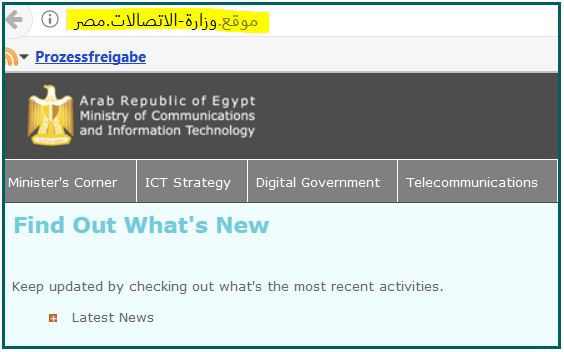
\includegraphics[width=\textwidth]{img/codierung_arabic.png}
        \end{column}
        \begin{column}{0.5\textwidth}
            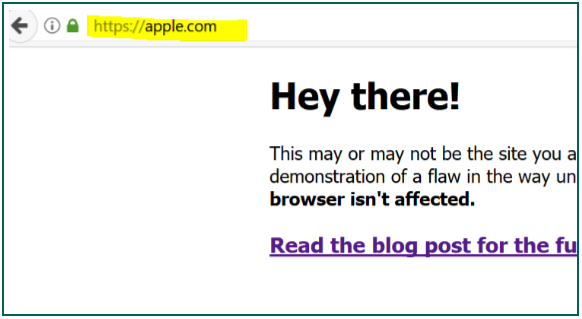
\includegraphics[width=\textwidth]{img/codierung_cyrillic_a.png}
        \end{column}
    \end{columns}
\end{frame}

\begin{frame}{Motivation 2: Numerische Zeichenreferenzen}
    \begin{alertblock}{\enquote{Problem}}
        \begin{itemize}
            \item HTML NCR: \&\#x5350; verweist auf Unicode-Codepoint
            \item Beispiel Swastika auf Google Trends
        \end{itemize}

    \end{alertblock}
    \begin{columns}
        \begin{column}{0.5\textwidth}
            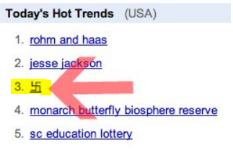
\includegraphics[width=\textwidth]{img/codierung_swastika_1.png}
        \end{column}
        \begin{column}{0.5\textwidth}
            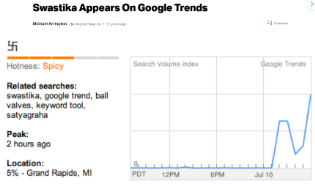
\includegraphics[width=\textwidth]{img/codierung_swastika_2.png}
        \end{column}
    \end{columns}
\end{frame}

\begin{frame}{Motivation 3: Sonderzeichen/Umlaute}
    \begin{block}{Anforderung}
        Wir wollen verschiedene Sprachen unterstützen
    \end{block}
    \begin{alertblock}{Problem}
        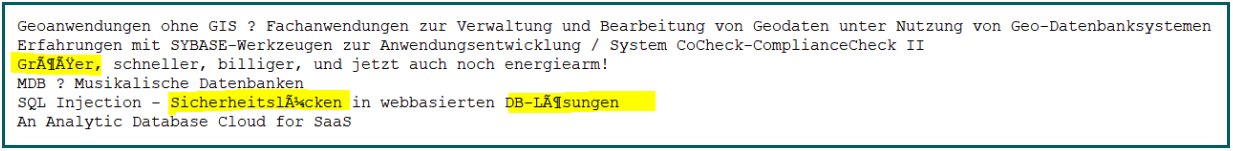
\includegraphics[width=\textwidth]{img/codierung_unicode_fail.png}
    \end{alertblock}
\end{frame}

\begin{frame}{Motivation 4: "Textbomben" / Unicode-Bugs}
    \begin{columns}
        \begin{column}{0.5\textwidth}
            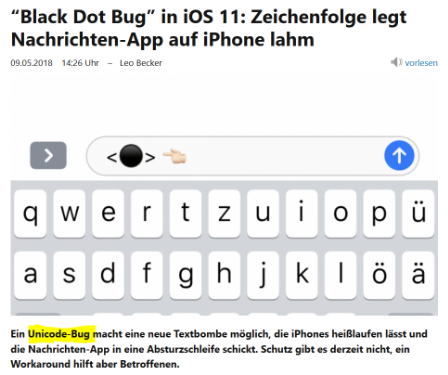
\includegraphics[width=\textwidth]{img/codierung_unicode_bomb_1.png}
        \end{column}
        \begin{column}{0.5\textwidth}
            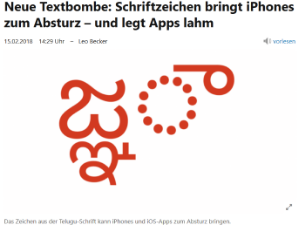
\includegraphics[width=\textwidth]{img/codierung_unicode_bomb_2.png}
        \end{column}
    \end{columns}
\end{frame}

% Section: Terminologie und Geschichte
\section{Terminologie und Geschichte}

\begin{frame}{Zeichenvorrat und Alphabet}
    \begin{block}{Definition: Zeichenvorrat (engl. Character Repertoire, CR)}
        Menge von Zeichen (ungeordnet)
        \begin{itemize}
            \item Menge aller Großbuchstaben (A, B, C, \dots, X, Y, Z)
                  \begin{itemize}
                      \item 26-elementiger Zeichenvorrat
                  \end{itemize}
            \item Menge aller Ziffern (0, 1, 2, \dots, 9)
                  \begin{itemize}
                      \item 10-elementiger Zeichenvorrat
                  \end{itemize}
            \item Binärer Zeichenvorrat
        \end{itemize}
    \end{block}
    \begin{block}{Defination: Alphabet}
        Geordneter Zeichenvorrat
    \end{block}
    \begin{block}{Definition Wort}
        Ein Wort $w$ der Länge $n$ über einen Zeichenvorrat $A$ ist eine endliche Folge $w = a_1 a_2 \ldots a_n \quad \vert \quad a_i \in A \mbox{ und } i \in \mathbb{N}$
    \end{block}
\end{frame}


\begin{frame}{Kurze Geschichte der Zeichencodierung}
    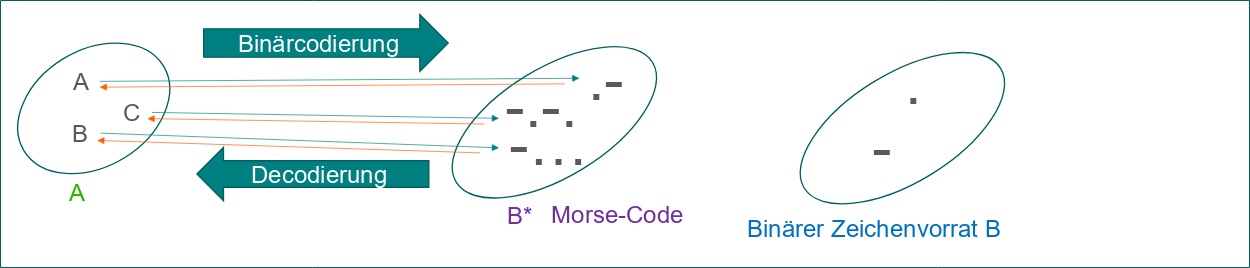
\includegraphics[width=\textwidth]{img/codierung_morsecode.png}
    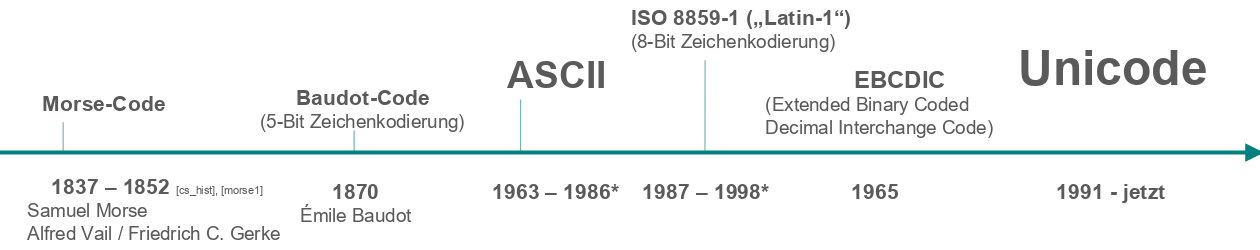
\includegraphics[width=\textwidth]{img/codierung_zeitstrahl.png}
\end{frame}

%\begin{frame}{Terminologie}{Zeichensatz vs. Zeichenkodierung}
%  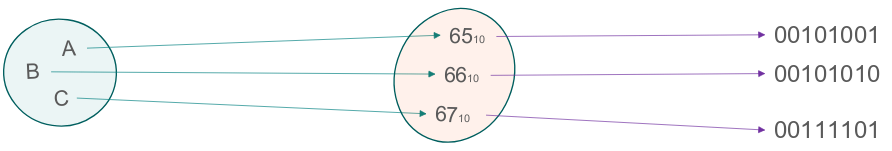
\includegraphics[width=\textwidth]{img/codierung_buchstabe_ccr_byte.png}
%  \begin{tabularx}{\textwidth}{lllX}
%    \toprule
%    Zeichenvorrat          & Zeichenvorrat                & Repräsentation/Bytes        & Definitionsgrundlage            \\
%    (ungeordnet)           & (geordnet)                   &                             &                                 \\
%    \midrule
%    Zeichensatz            & codierter Zeichensatz        & Zeichenkodierung            & World Wide Web Consortium (W3C) \\
%    \textit{Character Set} & \textit{Coded Character Set} & \textit{Character Encoding} &                                 \\
%    \midrule
%  \end{tabularx}
%
%
%\end{frame}

% Section: ASCII
\section{ASCII}


\begin{frame}{ASCII -- American Standard Code for Information Exchange}
    \begin{itemize}
        \item 95 druchbare Zeichen
        \item \textit{33 nicht druckbare Zeichen}
    \end{itemize}

    \begin{exampleblock}{ASCII-Table}
        \centering
        \setlength{\tabcolsep}{0.3em}
        \begin{tabular}{lcccccccccccccccc}
            \toprule
                        & \textbf{x0}  & \textbf{x1}  & \textbf{x2}  & \textbf{x3}  & \textbf{x4}  & \textbf{x5}  & \textbf{x6}  & \textbf{x7}  & \textbf{x8}  & \textbf{x9}       & \textbf{xA}       & \textbf{xB}  & \textbf{xC}      & \textbf{xD} & \textbf{xE} & \textbf{xF}  \\
            \midrule
            \textbf{0x} & \textit{NUL} & \textit{SOH} & \textit{STX} & \textit{ETX} & \textit{EOT} & \textit{ENQ} & \textit{ACK} & \textit{BEL} & \textit{BS}  & \textbackslash{}t & \textbackslash{}n & \textit{VT}  & \textit{FF}      & \textit{CR} & \textit{SO} & \textit{SI}  \\
            \textbf{1x} & \textit{DLE} & \textit{DC1} & \textit{DC2} & \textit{DC3} & \textit{DC4} & \textit{NAK} & \textit{SYN} & \textit{ETB} & \textit{CAN} & \textit{EM}       & \textit{SUB}      & \textit{ESC} & \textit{FS}      & \textit{GS} & \textit{RS} & \textit{US}  \\
            \textbf{2x} & SP           & !            & "            & \#           & \$           & \%           & \&           & '            & (            & )                 & *                 & +            & ,                & -           & .           & /            \\
            \textbf{3x} & 0            & 1            & 2            & 3            & 4            & 5            & 6            & 7            & 8            & 9                 & :                 & ;            & <                & =           & >           & ?            \\
            \textbf{4x} & @            & A            & B            & C            & D            & E            & F            & G            & H            & I                 & J                 & K            & L                & M           & N           & O            \\
            \textbf{5x} & P            & Q            & R            & S            & T            & U            & V            & W            & X            & Y                 & Z                 & [            & \textbackslash{} & ]           & \^{}        & \_           \\
            \textbf{6x} & `            & a            & b            & c            & d            & e            & f            & g            & h            & i                 & j                 & k            & l                & m           & n           & o            \\
            \textbf{7x} & p            & q            & r            & s            & t            & u            & v            & w            & x            & y                 & z                 & \{           & $a$              & \}          & $\sim$      & \textit{DEL} \\
            \bottomrule
        \end{tabular}
    \end{exampleblock}

\end{frame}

\begin{frame}[allowframebreaks]{ASCII -- American Standard Code for Information Exchange}{Nicht druckbare Buchstaben}
    \begin{description}
        \item[NUL] Null character, used to signify the end of a string.
        \item[SOH] Start of Header, used to indicate the start of a header in data transmission.
        \item[STX] Start of Text, marks the beginning of a text block.
        \item[ETX] End of Text, marks the end of a text block.
        \item[EOT] End of Transmission, used to signal the end of data transmission.
        \item[ENQ] Enquiry, used to request a response from a communication partner.
        \item[ACK] Acknowledge, indicates successful receipt of a message.
        \item[BEL] Bell, triggers an audible or visual signal.
        \item[BS] Backspace, moves the cursor one position backward.
        \item[HT] Horizontal Tab, moves the cursor to the next tab stop.
        \item[LF] Line Feed, moves the cursor to the next line.
        \item[VT] Vertical Tab, moves the cursor down to the next vertical tab stop.
        \item[FF] Form Feed, advances the paper to the top of the next page.
        \item[CR] Carriage Return, moves the cursor to the beginning of the line.
        \item[SO] Shift Out, switches to an alternate character set.
        \item[SI] Shift In, switches back to the standard character set.
        \item[DLE] Data Link Escape, used to indicate special control sequences.
        \item[DC1-DC4] Device Control 1-4, used for device-specific controls.
        \item[NAK] Negative Acknowledge, indicates a failure in data transmission.
        \item[SYN] Synchronous Idle, used to maintain synchronization between devices.
        \item[ETB] End of Transmission Block, indicates the end of a block of data.
        \item[CAN] Cancel, used to cancel the current operation.
        \item[EM] End of Medium, indicates the end of a storage medium.
        \item[SUB] Substitute, used to replace an invalid character.
        \item[ESC] Escape, introduces an escape sequence.
        \item[FS] File Separator, separates files in a data stream.
        \item[GS] Group Separator, separates groups of data.
        \item[RS] Record Separator, separates records in a data stream.
        \item[US] Unit Separator, separates units of data.
        \item[DEL] Delete, used to delete a character.
    \end{description}

\end{frame}

\begin{frame}[allowframebreaks]{ASCII -- American Standard Code for Information Exchange}{Eine nützliche Eigenschaft}
    \begin{columns}
        \begin{column}{0.5\textwidth}
            \begin{tabular}{cccc}
                \toprule
                Zeichen & Dezimal & Hexadezimal & Dual     \\
                \midrule
                A       & 65      & 41          & 01000001 \\
                B       & 66      & 42          & 01000010 \\
                \ldots  & \ldots  & \ldots      & \ldots   \\
                Y       & 89      & 59          & 01011001 \\
                Z       & 90      & 5A          & 01011010 \\
                \ldots  & \ldots  & \ldots      & \ldots   \\
                a       & 97      & 61          & 01100001 \\
                b       & 98      & 62          & 01100010 \\
                \ldots  & \ldots  & \ldots      & \ldots   \\
                y       & 121     & 79          & 01111001 \\
                z       & 122     & 7A          & 01111010 \\
                \bottomrule
            \end{tabular}
        \end{column}
        \begin{column}{0.5\textwidth}
            \begin{block}{Abstand zwischen Groß- und Kleinbuchstaben}
                \begin{itemize}
                    \item $A$ bis $Z$ = 65 bis 90
                    \item $a$ bis $z$ = 97 bis 122
                    \item Abstand = 32
                    \item Durch Addition von 32 kann ein Großbuchstabe in einen Kleinbuchstaben umgewandelt werden und umgekehrt.
                \end{itemize}
            \end{block}
        \end{column}
    \end{columns}
\end{frame}

% End document
\end{document}
